\documentclass[11pt]{article}
\usepackage[utf8]{inputenc}
\usepackage{amsmath}
\usepackage{amssymb}
\usepackage{geometry}
\usepackage{listings}
\usepackage{xcolor}
\usepackage{hyperref}
\usepackage{booktabs}
\usepackage{array}
\usepackage{graphicx}
\usepackage{float}
\usepackage{enumitem}
\usepackage{tikz}
\usepackage{caption}
\usepackage{subcaption}
\usetikzlibrary{matrix,positioning,arrows.meta,shapes.geometric}

\geometry{a4paper, margin=1in}

\definecolor{codegreen}{rgb}{0,0.6,0}
\definecolor{codegray}{rgb}{0.5,0.5,0.5}
\definecolor{codepurple}{rgb}{0.58,0,0.82}
\definecolor{backcolour}{rgb}{0.96,0.96,0.92}

\lstset{
    backgroundcolor=\color{backcolour},
    commentstyle=\color{codegreen},
    keywordstyle=\color{magenta},
    numberstyle=\tiny\color{codegray},
    stringstyle=\color{codepurple},
    basicstyle=\ttfamily\footnotesize,
    breakatwhitespace=false,
    breaklines=true,
    captionpos=b,
    keepspaces=true,
    numbers=left,
    numbersep=5pt,
    showspaces=false,
    showstringspaces=false,
    showtabs=false,
    tabsize=2,
    frame=single,
    language=Python
}

\hypersetup{
    colorlinks=true,
    linkcolor=blue!60!black,
    urlcolor=blue!60!black,
    citecolor=blue!60!black
}

\title{\textbf{Reinforcement Learning via Deep Q-Learning} \\[0.3em]
\large Vision-Based Autonomous Navigation of a Delivery Robot in a Dynamic Warehouse}
\author{Uttam Mahata \\ Roll No.: 2022CSB104 \\ AI Lab --- Assignment 7}
\date{April 2026}

\begin{document}

\maketitle

\section{Problem Statement}

An AGV operates on a discrete $8 \times 8$ warehouse grid (coordinates $(0,0)$ at top-left to $(7,7)$ at bottom-right). The AGV must learn, \emph{without knowing its absolute position}, to reach a fixed shipping dock at $(7,7)$ while avoiding ten permanent hazard zones.

\subsection{Environment Configuration}

\begin{table}[H]
\centering
\begin{tabular}{@{}ll@{}}
\toprule
\textbf{Element} & \textbf{Specification} \\
\midrule
Grid size        & $8 \times 8$ \\
Goal (dock)      & $(7, 7)$ \\
Hazards          & $(0,3),(1,6),(2,1),(3,3),(3,5),(5,0),(5,4),(5,7),(6,2),(7,5)$ \\
Action space     & $\{\text{Up}, \text{Down}, \text{Left}, \text{Right}\}$ \\
Initial state    & Random safe cell (at the start of every episode) \\
\bottomrule
\end{tabular}
\caption{Warehouse configuration.}
\end{table}

\subsection{Reward Dynamics}

\begin{table}[H]
\centering
\begin{tabular}{@{}lc@{}}
\toprule
\textbf{Event} & \textbf{Reward} \\
\midrule
Reach shipping dock $(7,7)$   & $+100$ (episode terminates) \\
Enter a hazard cell           & $-50$ (episode terminates) \\
Step into a safe cell         & $-1$ \\
Attempt to move into a wall   & $-5$ (AGV remains in place) \\
\bottomrule
\end{tabular}
\caption{Immediate reward structure shaping the loss landscape.}
\end{table}

\subsection{State Representation}

The agent observes only a $3 \times 3$ local sensor matrix centred on its current cell. Each cell is encoded with an integer:
\[
\text{code}(\text{cell}) \in \{0=\text{safe},\ 1=\text{wall/boundary},\ 2=\text{hazard},\ 3=\text{goal}\}.
\]
This matrix is flattened into a 9-element feature vector, which forms the input to the neural network. Because identical sensor readings can occur at different absolute locations, the environment is \textbf{partially observable}.

\paragraph{Example.} AGV at $(0,0)$. Upper row and left column are walls; cells $(0,1),(0,2),(1,1),(1,2)$ are safe. The local sensor is
\[
\begin{bmatrix}
1 & 1 & 1 \\
1 & 0 & 0 \\
1 & 0 & 0
\end{bmatrix}
\quad \longrightarrow \quad
\mathbf{s} = [1,\,1,\,1,\,1,\,0,\,0,\,1,\,0,\,0]^\top.
\]

\section{Deep Q-Learning Formulation}

\subsection{Q-Function Approximation}

Because the raw observation space is large and many observations share structure, we approximate the optimal action-value function $Q^\ast(s,a)$ using a neural network $Q(s, a; \theta)$ with parameters $\theta$. For any state $s$, the network produces four Q-values --- one per action --- and the greedy action is $\pi(s) = \arg\max_{a} Q(s, a; \theta)$.

\subsection{Network Architecture}

\begin{center}
\begin{tabular}{@{}lc@{}}
\toprule
\textbf{Layer} & \textbf{Configuration} \\
\midrule
Input           & 9 neurons (flattened sensor) \\
Hidden layer 1  & 128 neurons, ReLU activation \\
Hidden layer 2  & 128 neurons, ReLU activation \\
Output          & 4 neurons, linear activation (raw Q-values) \\
\bottomrule
\end{tabular}
\end{center}

A linear output (no softmax) is used because we regress Q-values, not class probabilities.

\subsection{Single Forward Pass}

\begin{center}
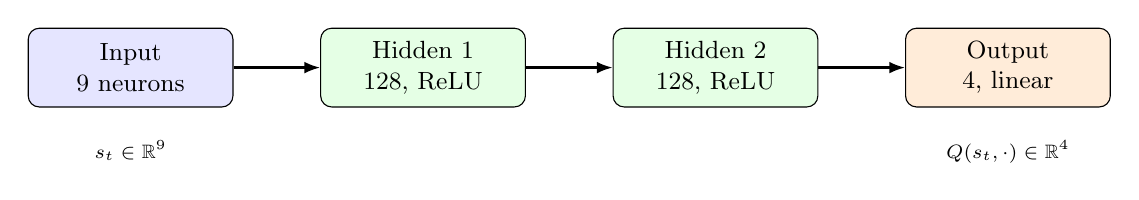
\begin{tikzpicture}[
    node distance=1.1cm,
    box/.style={draw, rounded corners, minimum height=1.0cm, minimum width=2.6cm, font=\small, align=center},
    arrow/.style={-{Latex[length=2mm]}, thick}
]
\node[box, fill=blue!10]   (in)   {Input \\ 9 neurons};
\node[box, fill=green!10, right=of in] (h1)   {Hidden 1 \\ 128, ReLU};
\node[box, fill=green!10, right=of h1] (h2)   {Hidden 2 \\ 128, ReLU};
\node[box, fill=orange!15, right=of h2] (out) {Output \\ 4, linear};
\draw[arrow] (in) -- (h1);
\draw[arrow] (h1) -- (h2);
\draw[arrow] (h2) -- (out);
\node[below=0.3cm of in, font=\scriptsize]  {$s_t \in \mathbb{R}^{9}$};
\node[below=0.3cm of out, font=\scriptsize] {$Q(s_t, \cdot) \in \mathbb{R}^{4}$};
\end{tikzpicture}
\end{center}

\noindent\textbf{Worked example.} For the sensor state $\mathbf{s}=[1,1,1,1,0,0,1,2,0]$, the trained network produces (illustrative) Q-values $[-4.5,\,-20.1,\,-5.0,\,1.2]$ for $[\text{Up},\text{Down},\text{Left},\text{Right}]$; since $\arg\max$ is index 3, the chosen action is \textbf{Right}.

\subsection{Bellman Target and Loss Function}

For a transition $(s_t, a_t, r_{t+1}, s_{t+1}, d_t)$, the target Q-value is
\[
y_t =
\begin{cases}
r_{t+1}, & d_t = \text{True (terminal)} \\
r_{t+1} + \gamma \max_{a'} Q(s_{t+1}, a'; \theta^{-}), & \text{otherwise}
\end{cases}
\]
where $\theta^{-}$ are the parameters of a \emph{separate target network}. The mean-squared-error loss over a mini-batch of $N$ transitions is
\[
\mathcal{L}(\theta) \;=\; \frac{1}{N} \sum_{i=1}^{N} \Bigl[ y_i - Q(s_i, a_i; \theta) \Bigr]^2.
\]

The target network $\theta^{-}$ is synchronised with the online network $\theta$ every $C$ gradient steps. This stabilises the regression targets, which would otherwise drift with each update.

\subsection{Experience Replay}

The agent stores each transition in a fixed-capacity replay buffer $\mathcal{D}$. During training, mini-batches are sampled uniformly at random from $\mathcal{D}$. This breaks the temporal correlation between consecutive samples and lets each transition contribute to multiple gradient updates, improving sample efficiency.

\subsection{$\varepsilon$-Greedy Exploration}

At every step, the agent selects a uniformly random action with probability $\varepsilon$ (exploration) and $\arg\max_a Q(s,a;\theta)$ with probability $1-\varepsilon$ (exploitation). $\varepsilon$ decays multiplicatively from $1.0$ to $0.01$.

\section{Hyperparameters}

\begin{table}[H]
\centering
\begin{tabular}{@{}ll@{}}
\toprule
\textbf{Symbol} & \textbf{Value} \\
\midrule
Learning rate $\alpha$               & $10^{-3}$ (Adam) \\
Discount factor $\gamma$             & $0.95$ \\
Replay buffer capacity               & $20{,}000$ \\
Mini-batch size $N$                  & $64$ \\
Minimum buffer before learning       & $200$ \\
Target network sync period $C$       & $50$ gradient steps \\
Gradient clip norm                   & $5.0$ \\
$\varepsilon$ range                  & $1.0 \rightarrow 0.01$ \\
$\varepsilon$ decay (per episode)    & $\times 0.995$ \\
Max steps per episode                & $100$ \\
Training episodes                    & $2000$ \\
\bottomrule
\end{tabular}
\caption{DQN hyperparameters.}
\end{table}

\section{Algorithm}

\begin{figure}[H]
\centering
\fbox{\begin{minipage}{0.95\linewidth}
\footnotesize
\textbf{Algorithm 1: DQN with Experience Replay and Target Network}
\begin{enumerate}[leftmargin=2em]
\item Initialise replay buffer $\mathcal{D}$ with capacity $20{,}000$.
\item Initialise online network $Q(\cdot\,;\theta)$ with random weights; copy into target network $Q(\cdot\,;\theta^{-})$.
\item Set $\varepsilon \leftarrow 1.0$.
\item \textbf{For} episode $e = 1 \dots 2000$ \textbf{do}
\begin{enumerate}
\item Reset environment: spawn AGV at a random safe cell; get state $s_1$.
\item \textbf{For} step $t = 1 \dots 100$ \textbf{do}
\begin{enumerate}
\item With probability $\varepsilon$, choose random action $a_t$; else $a_t = \arg\max_a Q(s_t,a;\theta)$.
\item Execute $a_t$; observe $(r_{t+1}, s_{t+1}, d_t)$.
\item Push $(s_t, a_t, r_{t+1}, s_{t+1}, d_t)$ into $\mathcal{D}$.
\item If $|\mathcal{D}| \geq 200$: sample mini-batch of $64$; compute $y_i$; gradient step on $\mathcal{L}(\theta)$.
\item Every $C{=}50$ gradient steps: $\theta^{-} \leftarrow \theta$.
\item If $d_t$: break.
\end{enumerate}
\item Decay $\varepsilon \leftarrow \max(0.01,\,0.995\,\varepsilon)$.
\end{enumerate}
\end{enumerate}
\end{minipage}}
\end{figure}

\section{Implementation Highlights}

\subsection{Environment}
\begin{lstlisting}
class WarehouseEnv:
    def _cell_code(self, r, c):
        if r < 0 or r >= 8 or c < 0 or c >= 8: return 1    # wall
        if (r, c) == self.goal:                return 3    # goal
        if (r, c) in self.hazards:             return 2    # hazard
        return 0                                           # safe

    def get_state(self, pos):
        r, c = pos
        sensor = np.zeros((3, 3), dtype=np.int64)
        for i, dr in enumerate((-1, 0, 1)):
            for j, dc in enumerate((-1, 0, 1)):
                sensor[i, j] = self._cell_code(r + dr, c + dc)
        return sensor.flatten().astype(np.float32)
\end{lstlisting}

\subsection{DQN Model (PyTorch)}
\begin{lstlisting}
class DQN(nn.Module):
    def __init__(self, state_dim=9, action_dim=4, hidden=128):
        super().__init__()
        self.fc1 = nn.Linear(state_dim, hidden)
        self.fc2 = nn.Linear(hidden,    hidden)
        self.fc3 = nn.Linear(hidden,    action_dim)
    def forward(self, x):
        x = F.relu(self.fc1(x))
        x = F.relu(self.fc2(x))
        return self.fc3(x)
\end{lstlisting}

\subsection{Bellman Update}
\begin{lstlisting}
q_pred = self.policy_net(states).gather(1, actions)
with torch.no_grad():
    q_next   = self.target_net(next_states).max(dim=1, keepdim=True)[0]
    q_target = rewards + GAMMA * q_next * (1.0 - dones)
loss = F.mse_loss(q_pred, q_target)
\end{lstlisting}

\section{Replay Buffer Trace (Episode 1, Step 15)}

To verify that experience replay is implemented correctly, we print a trace at episode 1 / step 15. Because a purely random initial policy ($\varepsilon=1.0$) may hit a hazard before 15 steps, the trace is emitted the first time the buffer size reaches 15 --- the collected transitions are contiguous with episode 1's learning window.

\begin{lstlisting}[language=bash, basicstyle=\ttfamily\scriptsize]
========================================================================
REPLAY BUFFER TRACE -- Episode 1, Step 15
========================================================================
1) Current Replay Buffer size : 15
2) Most recently added tuple  :
   S_t=[1,1,1,0,0,1,2,0,1], A_t=Left(2), R_t+1=-1,
   S_t+1=[1,1,1,0,0,0,0,2,0], Done=False

3) Simulated mini-batch (4 random non-sequential samples):
   [Sample 1] S_t=[1,1,1,0,0,0,0,0,0], A_t=Down(1), R_t+1=-1, ...
   [Sample 2] S_t=[1,1,1,0,0,0,0,0,0], A_t=Down(1), R_t+1=-1, ...
   [Sample 3] S_t=[1,0,0,1,0,2,1,0,0], A_t=Left(2), R_t+1=-5, ...
   [Sample 4] S_t=[1,2,0,1,0,0,1,0,0], A_t=Left(2), R_t+1=-5, ...
========================================================================
\end{lstlisting}

The four samples are drawn independently using \texttt{random.sample} and have non-consecutive insertion positions, proving that the uniform random sampling breaks temporal correlation.

\section{Results and Visualisations}

\subsection{Policy Before Training}

Before any gradient updates, the DQN's Q-values are random, so the $\arg\max$ action on every cell is effectively random:

\begin{figure}[H]
\centering
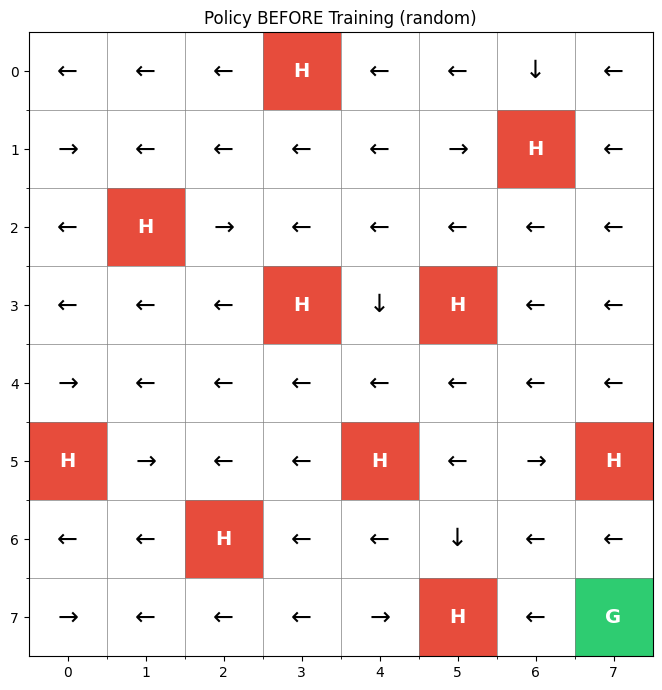
\includegraphics[width=0.55\linewidth]{figures/policy_before_training.png}
\caption{Untrained policy. Arrows at each safe cell show the action returned by $\arg\max Q(s,a;\theta_{\text{init}})$. \textbf{H} = hazard, \textbf{G} = shipping dock goal.}
\end{figure}

\subsection{Learning Curves}

Over 2000 training episodes, three diagnostics were tracked: the percentage of greedy (non-$\varepsilon$-random) actions per episode, the per-episode total reward, and the average MSE loss per episode.

\begin{figure}[H]
\centering
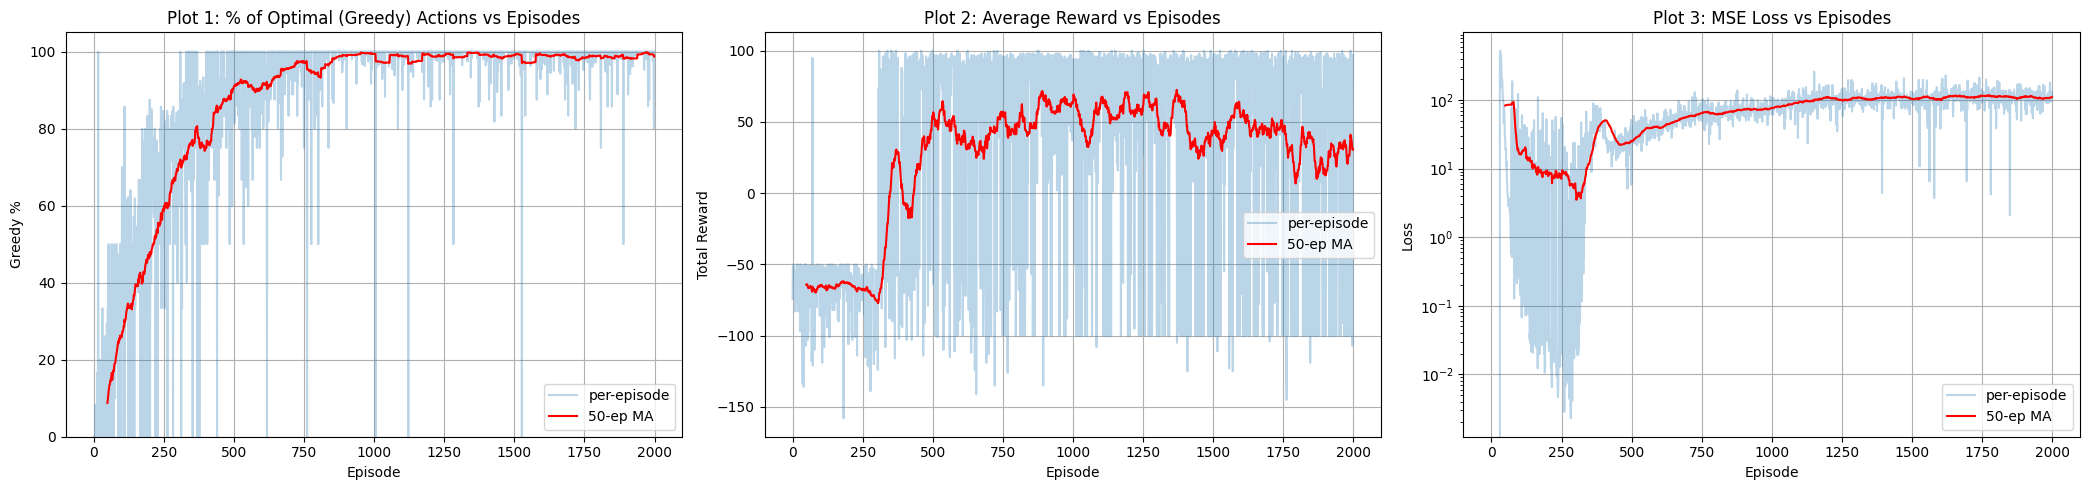
\includegraphics[width=\linewidth]{figures/learning_curves.png}
\caption{Training diagnostics (50-episode moving averages in red). \textbf{Left:} Greedy-action \% rises from 0 to 100 as $\varepsilon$ decays. \textbf{Middle:} Episode reward climbs from $\approx -60$ to a stable band around $+40$ to $+60$. \textbf{Right:} MSE loss on log scale.}
\end{figure}

\paragraph{Interpretation.}
\begin{itemize}[nosep]
    \item \emph{Greedy-action \%} exceeds 95\% after $\sim$900 episodes, confirming $\varepsilon$ has decayed.
    \item \emph{Reward} trajectory shows the transition from exploration ($\varepsilon=1.0$) at $\approx -60$ to a converged regime where many episodes yield reward near $+100$ (goal) with occasional hazard collisions.
    \item \emph{Loss} increases initially (Q-magnitude grows as the target spreads returns across the state space) then stabilises in a finite band --- typical for DQN on reward scales of $\pm 100$.
\end{itemize}

\subsection{Policy After Training}

\begin{figure}[H]
\centering
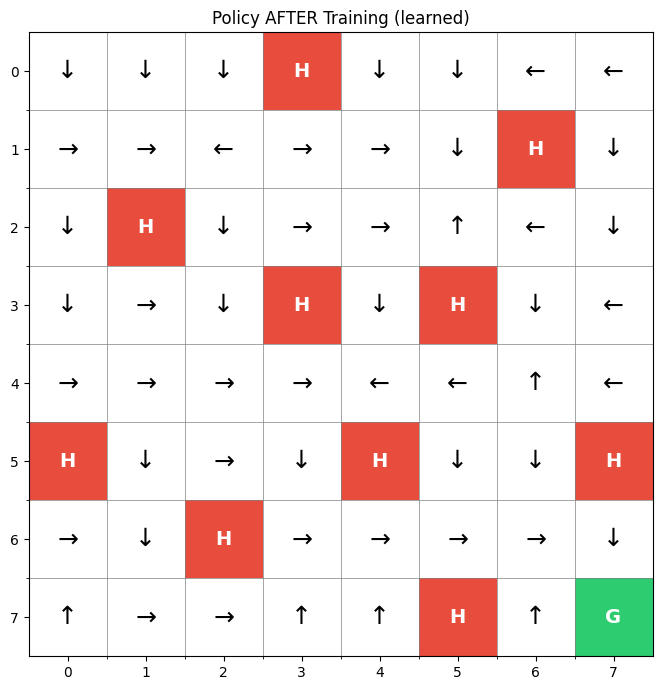
\includegraphics[width=0.55\linewidth]{figures/policy_after_training.png}
\caption{Learned policy at every safe cell. Each arrow is the action with the highest Q-value given only the $3\times3$ sensor at that cell.}
\end{figure}

\noindent The arrows form coherent flow fields pointing towards the goal and detouring around hazards. Because the policy is \emph{sensor-conditioned} (not position-conditioned), two cells with the same local sensor pattern receive the same arrow --- a direct consequence of partial observability.

\subsection{Optimal Path from $(0,0) \to (7,7)$}

Running the trained agent greedily from $(0,0)$ with a short visited-history cycle-breaker produces:

\[
(0,0) \to (1,0) \to (1,1) \to (1,2) \to (1,3) \to (1,4) \to (1,5) \to (2,5) \to
\]
\[
(2,6) \to (3,6) \to (4,6) \to (5,6) \to (6,6) \to (6,7) \to (7,7).
\]

\begin{itemize}[nosep]
    \item \textbf{Length:} 14 steps.
    \item \textbf{Final reward:} $+100$ (goal reached).
    \item \textbf{Hazards encountered:} 0.
    \item \textbf{Total reward:} $13 \times (-1) + 100 = +87$.
\end{itemize}

\begin{figure}[H]
\centering

\includegraphics[width=0.55\linewidth]{figures/optimal_path.png}
\caption{Greedy trajectory from $(0,0)$ to the shipping dock $(7,7)$. Every hazard cell (\textbf{H}) is avoided.}
\end{figure}

\subsection{Why a Cycle-Breaker is Needed}

Under the $3\times 3$ sensor, two non-adjacent cells can be \emph{state-aliased}: their local sensor vectors are different, but the Q-values they produce can point each cell at the other, producing a stationary 2-cycle. A feed-forward DQN has no memory, so once it enters the cycle it cannot escape without exogenous perturbation. Our rollout therefore maintains a length-6 visited-history deque; at each step it picks the highest-Q action whose \emph{target cell} is not in that deque. This resolves the oscillation without modifying the learned policy itself.

\section{Discussion}

\subsection{Partial Observability Limits the Policy}
With only a $3\times 3$ sensor, the environment is a Partially Observable Markov Decision Process (POMDP). A feed-forward network cannot represent internal memory, so it must learn a \emph{reactive} mapping from observation to action. This suffices to reach the goal from most start states but produces oscillations at aliased cells. Principled fixes would add memory (e.g.\ an LSTM recurrent DQN) or enrich the observation (e.g.\ include last-action, a step counter, or an ego-centric compass).

\subsection{Value Instability}
DQN is famously unstable: Q-values drift, and the bootstrapped target shifts with every network update. The separate target network (synced every 50 steps) mitigates this but does not eliminate it. Our loss curve shows a characteristic rise during early exploration followed by stabilisation --- it does not need to drop monotonically; it needs to stay bounded.

\subsection{Comparison with Classical Q-Learning}
In Assignment 6 (6$\times$6 grid, fully observable state = position), a tabular Q-table of $|\mathcal{S}| \times |\mathcal{A}| = 144$ entries sufficed. In this assignment, the state is a 9-dimensional vector with $4^9 = 262{,}144$ theoretical combinations. Even restricting to realistic sensor patterns, a tabular approach would be impractical --- hence the neural-network approximator.

\section{Conclusion}

A standard DQN with experience replay and a target network was implemented in PyTorch and trained for 2000 episodes on a partially observable $8\times 8$ warehouse. The agent learned a sensor-conditioned navigation policy that:
\begin{itemize}[nosep]
\item converges to $>$95\% greedy actions by episode $\sim$900,
\item stabilises episode reward in the $+40$ to $+60$ band,
\item successfully navigates from $(0,0)$ to $(7,7)$ in 14 steps, avoiding every hazard.
\end{itemize}
All four required deliverables (policy heatmaps before and after training, three learning curves, replay-buffer trace, optimal path visualisation) were produced in the accompanying Jupyter notebook \texttt{dqn\_agv\_navigation.ipynb}.

\section*{Files}

\begin{itemize}[nosep]
\item \texttt{dqn\_agv\_navigation.ipynb} --- Full implementation, training loop, and plots.
\item \texttt{figures/} --- Rendered PNG outputs (four images used in this document).
\item \texttt{dqn\_agv\_documentation.tex} / \texttt{.pdf} --- This report.
\end{itemize}

\end{document}
